\graphicspath{ {../../images/} }
\usetikzlibrary{external}
\usepackage{pifont}

% Needed for the distinguishing game
\usepackage{crygame}

\title{ICS0036 Cryptography}
\subtitle{Randomness, OTP, and stream ciphers}
\date{\today}
\author{Taaniel Kraavi}
\institute%
{%
  \textit{IT College}\\
  \textit{Tallinn University of Technology}
}

\begin{document}
\begin{frame}
  \titlepage
\end{frame}

\begin{frame}
  \frametitle{Is it random?}

  \begin{itemize}
    \item<1-> 2204219747
    \begin{itemize}
      \item<2-> \texttt{10000011 01100001 10111001 01100011}
      \item<2-> \texttt{0}: $17$, \texttt{1}: $15$
      \item<3-> Source: \texttt{/dev/urandom}
    \end{itemize}
    \item<1-> 1415926535
    \begin{itemize}
      \item<2-> \texttt{01010100 01100101 01010011 00000111}
      \item<2-> \texttt{0}: $18$, \texttt{1}: $14$
      \item<4-> Source: first 10 decimal digits of $\pi$
    \end{itemize}
    \item<1-> 1918987876
    \begin{itemize}
      \item<2-> \texttt{01110010 01100001 01101110 01100100}
      \item<2-> \texttt{0}: $17$, \texttt{1}: $15$
      \item<5-> Source: decoded ASCII string \enquote{rand}
    \end{itemize}
  \end{itemize}
\end{frame}

\begin{frame}
  \frametitle{XKCD 221}

  \begin{figure}
    \centering
    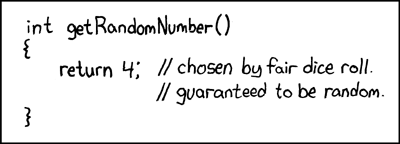
\includegraphics[height=80px]{xkcd221.png}
    \caption{\url{https://xkcd.com/221/}}
  \end{figure}
\end{frame}

\begin{frame}
  \frametitle{Randomness}

  % Mention double pendulums, Cloudflare lava lamps
  \begin{itemize}[<+->]
    \item Randomness is unprovable
    \item Statistical tests for non-randomness
    \item \enquote{True} randomness:
    \begin{itemize}
      \item Thermal noise, photoelectric effect, quantum phenomena, \dots
    \end{itemize}
    \vspace*{1em}
    \item Random sequence
    \begin{itemize}
      \item forward \& backward unpredictable
      \item follows no deterministic pattern
      \item cannot be compressed
      \item has no description shorter than itself
    \end{itemize}
    \vspace*{1em}
    \item Computers and humans are predictable
  \end{itemize}
\end{frame}

\begin{frame}
  \frametitle{Randomness in cryptography}

  High quality randomness is crucial in cryptography:
  \begin{itemize}[<+(1)->]
    \item secret values (e.g. secrecy of keys)
    \item uniqueness (e.g. single use values/tokens (nonces))
  \end{itemize}
\end{frame}

\begin{frame}
  \frametitle{RNG}

  RNG: random number generator
  \begin{itemize}[<+(1)->]
    \item The term is often used loosely
    \item More precise terminology:
    \begin{itemize}
      \item hardware, true \& quantum RNG: HRNG, TRNG, QRNG
      \item NRBG: non-deterministic random bit generator
    \end{itemize}
  \end{itemize}

  \vspace*{1em}

  \pause
  In cryptography, we consider TRNGs.
\end{frame}

\begin{frame}
  \frametitle{TRNG}

  \pause
  A TRNG requires a physical source of \emph{entropy}.
  \begin{itemize}[<+(1)->]
    \item Entropy (in computing): amount of unpredictable randomness
    \item Therefore, entropy must be collected
  \end{itemize}

  \vspace*{1em}

  \pause
  Entropy sources:
  \begin{itemize}[<+(1)->]
    \item Integrated (opaque)
    \item External (more choice)
  \end{itemize}
\end{frame}

\begin{frame}
  \frametitle{Entropy pool}

  \pause
  How do computers fill the entropy pool?
  \begin{itemize}[<+(1)->]
    \item Entropy is collected and (typically) accumulated in a pool
    \item Hardware sources, interrupt signals, user behaviour, \dots
  \end{itemize}

  \vspace*{1em}

  \pause
  Quality/quantity of entropy:
  \begin{itemize}[<+(1)->]
    \item Beware of boot: low entropy
    \item Amount of entropy / collection throughput?
    \item To block or not to block?
  \end{itemize}

  \vspace*{1em}

  \pause
  Do we always need a TRNG?
\end{frame}

% \begin{frame}
%   \frametitle{RNG}

%   \begin{itemize}[<+->]
%     \item Random number generators
%     \item RNG boogaloo:
%     \begin{itemize}
%       \item hardware, true \& quantum RNG: HRNG, TRNG, QRNG
%       \item NRBG: non-deterministic random bit generator
%     \end{itemize}
%     \item HRNG requires a physical source of entropy
%     \begin{itemize}
%       \item Integrated (opaque)
%       \item External (more choice)
%     \end{itemize}
%     \item How do computers fill the entropy pool?
%     \begin{itemize}
%       \item Hardware sources, interrupt signals, user behaviour, \dots
%       \item Beware of boot: low entropy
%       \item Quantity of entropy?
%       \item To block or not to block?
%     \end{itemize}
%     \item Do we always need a TRNG?
%   \end{itemize}
% \end{frame}

\begin{frame}
  \frametitle{PRNG}

  PRNG: pseudo-random number generator
  \begin{itemize}[<+(1)->]
    \item More precise terminology:
    \begin{itemize}
      \item CSPRNG: cryptographically secure PRNG
      \item DRBG: deterministic random bit generator
    \end{itemize}
    \item Deterministic
    \item Random input \emph{seed}
  \end{itemize}

  \vspace*{1em}

  \pause
  Best practice: CSPRNG seeded (and reseeded) by a TRNG.
  \begin{itemize}[<+(1)->]
    \item Suitable for most (cryptographic) uses.
    \item A CSPRNG does not protect against a poor seed.
  \end{itemize}
\end{frame}

\begin{frame}
  \frametitle{Resources}

  Some recommendations/standards:
  \begin{itemize}
    \item \href{https://csrc.nist.gov/projects/random-bit-generation}{NIST on random bit generation}
    \begin{itemize}
      \item \url{https://csrc.nist.gov/projects/random-bit-generation}
    \end{itemize}
    \item \href{https://www.bsi.bund.de/dok/randomnumbergenerators}{BSI on random number generators}
    \begin{itemize}
      \item \url{https://www.bsi.bund.de/dok/randomnumbergenerators}
    \end{itemize}
  \end{itemize}
\end{frame}

\begin{frame}
  \frametitle{An intuition on construction}

  We want a black box with:
  \begin{itemize}[<+(1)->]
    \item \enquote{confusion}
    \item diffusion (avalanche effect)
  \end{itemize}

  \pause
  Given this black box:
  \begin{itemize}[<+(1)->]
    \item compute one output \enquote{block} from the seed and counter
    \item increment the counter
    \item repeat as needed
  \end{itemize}

  \pause
  This is one type of construction, but there are others.
\end{frame}

\begin{frame}
  \frametitle{Getting randomness on *nix}

  \pause
  Device files:
  \begin{itemize}
    \item \texttt{/dev/random}: historically blocking, but not any more ($\ge$ kernel 5.6)
    \item \texttt{/dev/urandom}: historically non-blocking
    \pause
    \item Both are a CSPRNG outputs seeded from the entropy pool
    \pause
    \item Documentation is commonly obsolete
    \pause
    \item Beware of flavour/kernel differences!
  \end{itemize}

  \vspace*{1em}
  
  \pause
  Beware of randomness in VMs!
  \begin{itemize}
    \item A nice \href{https://blogs.oracle.com/linux/post/rngd1}{\emph{blog post}} by Oracle.
  \end{itemize}
\end{frame}

\begin{frame}{Platform functions}
  \begin{itemize}[<+(1)->]
    \item Linux: \href{https://man7.org/linux/man-pages/man2/getrandom.2.html}{\texttt{getrandom()}}
    \begin{itemize}
      \item \texttt{GRND\_RANDOM} flag for \texttt{random} vs \texttt{urandom}
      \item Beware of obsolete documentation (e.g. \texttt{GRND\_NONBLOCK} flag)!
    \end{itemize}
    \vspace*{1em}
    \item macOS: \href{https://developer.apple.com/documentation/security/secrandomcopybytes(_:_:_:)}{\texttt{SecRandomCopyBytes}}
    \vspace*{1em}
    \item Windows: \href{https://learn.microsoft.com/en-us/windows/win32/api/bcrypt/nf-bcrypt-bcryptgenrandom}{\texttt{BCryptGenRandom}}
    \begin{itemize}
      \item \href{https://learn.microsoft.com/en-us/windows/win32/api/wincrypt/nf-wincrypt-cryptgenrandom}{\texttt{CryptGenRandom}} is being deprecated
      \item For .NET, use \href{https://learn.microsoft.com/en-us/dotnet/api/system.security.cryptography.randomnumbergenerator}{\texttt{RandomNumberGenerator}}
      \item \href{https://learn.microsoft.com/en-us/dotnet/api/system.security.cryptography.rngcryptoserviceprovider}{\texttt{RNGCryptoServiceProvider}} is deprecated
    \end{itemize}
  \end{itemize}
\end{frame}

\begin{frame}{PRNG security (informal)}
  \pause
  The output of a CSPRNG should be \emph{indistinguishable} from true randomness to a \emph{computationally bounded} adversary.
  \begin{enumerate}[<+(1)->]
    \item The challenger selects one of the two algorithms:
    \begin{align*}
      &\begin{game}{\GAME_0}
        &r\getsu\{0,1\}^\ell\\
        &\RETURN r
      \end{game}
      &\begin{game}{\GAME_1}
        &s\getsu\{0,1\}^k\\
        &r\gets\mathsf{CSPRNG}(s, \ell)\\
        &\RETURN r
      \end{game}
    \end{align*}
    \item The adversary queries the challenger for the $\ell$-bit output $r$.
    \item The adversary announces which algorithm they think is used.
  \end{enumerate}

  \pause
  If the adversary is correct only about half the time, we consider the CSPRNG to be \enquote{secure}.
\end{frame}

\begin{frame}
  \frametitle{Trusting randomness}

  \pause
  Mixing entropy sources
  \begin{itemize}[<+(1)->]
    \item Integrated \& external (speed boost)
    \item Client \& server-side
    % Explain that this is sometimes bad.
    % \item Combine with timestamp (helps with bad randomness)
    \item Mixing has gotchas!
  \end{itemize}

  \vspace*{0.5em}

  \pause
  DYOR:
  \begin{itemize}[<+(1)->]
    \item Is it open source?
    \item Certified?
    \item Reputable vendor?
    \item Track record?
  \end{itemize}

  \vspace*{0.5em}

  \pause
  Randomness combined with anything\textsuperscript{*} is random.
  {\scriptsize \textsuperscript{*}without information loss}
\end{frame}

\begin{frame}
  \frametitle{XOR}

  \pause
  XOR ($\oplus$): exclusive OR
  \pause
  \begin{displaymath}
    \begin{array}{|c|c|c|}
      a & b & a \oplus b\\
      \hline
      0 & 0 & 0\\
      0 & 1 & 1\\
      1 & 0 & 1\\
      1 & 1 & 0\\
    \end{array}
  \end{displaymath}

  \pause
  Reversible\textsuperscript{*} without information loss:
  \begin{columns}[T]
    \begin{column}{.5\textwidth}
      \begin{itemize}[<+(1)->]
        \item associative: $a \oplus (b \oplus c) = (a \oplus b) \oplus c$
        \item commutative: $a \oplus b = b \oplus a$
      \end{itemize}
    \end{column}
    \begin{column}{.5\textwidth}
      \begin{itemize}[<+(1)->]
        \item self-inverse: $a \oplus a = 0$
        \item identity element: $a \oplus 0 = a$
      \end{itemize}
    \end{column}
  \end{columns}

  \vspace*{1em}

  {\scriptsize \textsuperscript{*} knowing the output and an input}
\end{frame}

\begin{frame}
  \frametitle{One-time pad (OTP)}

  Symmetric, deterministic cryptosystem
  \begin{columns}[T]
    \begin{column}{0.55\textwidth}
      \pause
      \begin{itemize}
        \item Same key for encryption and decryption
        \item One ciphertext for each message
      \end{itemize}
    \end{column}
    \begin{column}{0.378\textwidth}
      \pause
      \begin{itemize}
        \item $\ENC_k(m) = m \oplus k = c$
        \item $\DEC_k(c) = c \oplus k = m$
      \end{itemize}
    \end{column}
  \end{columns}

  \vspace*{1em}

  \pause
  The $\lambda$-bit key $k$ must:
  \begin{itemize}[<+(1)->]
    \item $k \getsu \{0,1\}^\lambda$, i.e. be sampled uniformly at random (\enquote{perfectly} random)
    \item $\lambda \ge \lvert m\rvert$, i.e. be (at least) as long as the message 
    \item be used only once
  \end{itemize}
\end{frame}

\begin{frame}
  \frametitle{One-time pad (OTP)}
  The OTP is \textbf{information theoretically secure}, i.e. it has \emph{perfect secrecy}.
  \begin{itemize}[<+(1)->]
    \item No bit of information is leaked
    \item All decryptions are valid $\iff$ the intended message cannot be identified
    \item Brute force alone is useless even for an \emph{unbounded} adversary
  \end{itemize}

  \vspace*{1em}

  \pause
  \begin{center}
    {\color{red} Catastrophic failure if any of the 3 conditions is not respected!}
  \end{center}
\end{frame}

\begin{frame}
  \frametitle{OTP limitations}

  \pause
  Size issues:
  \pause
  \begin{itemize}
    \item Key as long as the message
    \item How do we design and store the codebook?
  \end{itemize}

  \pause
  Practicality issues:
  \pause
  \begin{itemize}
    \item New key for every message
    \item How do we synchronise keys and exchange the codebook?
  \end{itemize}

  \pause
  Security issues:
  \pause
  \begin{itemize}
    \item No authenticity/integrity
    \item \emph{Malleable}, i.e. can be meaningfully altered
  \end{itemize}
\end{frame}

\begin{frame}
  \frametitle{Symmetric cryptosystems}

  A \emph{private-key encryption scheme} is a triple of algorithms:
  \begin{itemize}
    \pause\item $\GEN$ is a randomised \emph{key generation algorithm}: $k\gets\GEN$
    \pause\item $\ENC$ is a (possibly randomised) \emph{encryption algorithm}: $c\gets\ENC_k(m)$
    \pause\item $\DEC$ is a \emph{decryption algorithm}: $m\gets\DEC_k(c)$.
  \end{itemize}

  \vspace*{1em}

  \begin{itemize}
    \pause\item $k$ is the \emph{private key}, also called \emph{secret key}
    \pause\item The message $m$ is the \emph{plaintext}
    \pause\item The encrypted message $c$ is the \emph{ciphertext}
  \end{itemize}

  \vspace*{1em}

  \pause
  The cryptosystem is \emph{functional} (achieves \emph{correctness}) if $\DEC_k(\ENC_k(m))=m$.
\end{frame}

\begin{frame}
  \frametitle{Symmetric cryptosystems}
  \framesubtitle{For mathematical rigour}

  Keys, messages, and ciphertexts must belong to \emph{spaces}, i.e. sets of elements:
  \begin{itemize}
    \pause\item Key space $\KKK$
    \pause\item Message space $\MMM$
    \pause\item Ciphertext space $\CCC$
  \end{itemize}

  \vspace*{1em}

  \pause
  The functions are therefore maps
  \begin{itemize}
    \pause\item $\ENC_k:\MMM\to\CCC$
    \pause\item $\DEC_k:\CCC\to\MMM\cup\{\bot\}$
  \end{itemize}

  \vspace*{1em}

  \pause
  The symbol $\bot$ (\enquote{bottom}) denotes decryption failure, i.e. the \emph{abort} symbol. 
\end{frame}

\begin{frame}{Symmetric cryptosystems}
  \framesubtitle{EAV-security}
  \begin{center}
  \begin{tikzpicture}
    \node (alice) at (0,0)      {\includegraphics[height=80px]{alice}};
    \node (bob)   at (8, 0)     {\includegraphics[height=80px]{bob}};
    \node (eve)   at (4, -2.1)  {\includegraphics[height=80px]{eve}};

    \draw[->,thick] (alice.east) -- (bob.west);
    \draw[->,thick] (4, 0) -- (4, -0.5);
    \node[anchor=center,draw,circle,fill=white,thick,minimum size = 2px, inner sep=0pt] at (4,0) {};
    
    \node (c) at (4, 0.2) {$c$};
    \node (gen)   at (4, 2) {$\GEN$};

    \node (ska) at (alice.north) [xshift=-7px,yshift=7px] {$k$};
    \node (skb) at (bob.north) [xshift=7px,yshift=7px] {$k$};

    \draw[<-,dashed,thick] (alice.north) |- (gen.west);
    \draw[->,dashed,thick] (gen.east) -| (bob.north);

    \node[anchor=west] (m) at (-3, 0.25) {$m\gets\MMM$};
    \node[anchor=west] (enc) at (-3, -0.25) {$c\gets\ENC_k(m)$};
    \node[anchor=east] (dec) at (11, 0) {$m\gets\DEC_k(c)$};
  \end{tikzpicture}
  \end{center}

  \pause
  Can Eve guess the message that Alice sent Bob?
\end{frame}

\begin{frame}
  \frametitle{Semantic security (informal)}

  Cryptographers speak of \emph{semantic security}.
  \begin{itemize}[<+(1)->]
    \item Knowing a ciphertext is no more useful than only knowing its length
    \item Computational equivalent to perfect secrecy
  \end{itemize}

  \vspace*{1em}

  \pause
  Semantic security is difficult to work with.
  \begin{itemize}[<+(1)->]
    \item We aim for CPA-\emph{indistinguishability} instead
    \item IND-CPA $\implies$ IND-SEM
  \end{itemize}
\end{frame}

\begin{frame}
  \frametitle{IND-CPA (informal)}

  The scheme has IND-CPA if a computationally bounded adversary cannot distinguish which of two messages was encrypted.
  \begin{enumerate}[<+(1)->]
    \item The adversary prepares and sends two messages $m_0, m_1$ of equal size to the challenger.
    \item The challenger randomly selects either $m_0$ or $m_1$, encrypts it, and sends the ciphertext to the adversary.
    \item The adversary announces which message they think was encrypted.
  \end{enumerate}

  \pause
  If the adversary is correct only about half the time, we consider the cryptosystem to have IND-CPA.
\end{frame}

\begin{frame}{Stream ciphers (conceptually)}
  Follows from the OTP:
  \begin{itemize}[<+(1)->]
    \item Symmetric cipher
    \item The key is the \emph{seed} of a PRNG
    \item XORs the message with the PRNG stream: the \emph{keystream}
  \end{itemize}

  \vspace*{1em}

  \pause
  How to decrypt?
  \begin{itemize}[<+(1)->]
    \item Recipient re-generates the keystream from the seed (key)
    \item Recipient XORs the ciphertext with the keystream
  \end{itemize}

  \vspace*{1em}

  \pause
  What happens when you encrypt multiple messages with the same key?
\end{frame}

\begin{frame}{Stream cipher nonce}
  Goal: keep the key, but use a unique keystream per encryption

  \pause
  For each encryption:
  \begin{enumerate}[<+(1)->]
    \item Generate a \emph{nonce} (unique value)
    \item Initialise the cipher with the key and fresh nonce
    \item Send the (nonce, ciphertext) pair to the recipient
  \end{enumerate}

  \pause
  The nonce:
  \begin{itemize}[<+(1)->]
    \item Is \emph{not} secret
    \item Must be freshly selected for each encryption
    \item Must \emph{not} be reused under the same key
    \begin{itemize}
      \item Easiest way: use a \enquote{long enough} nonce to statistically avoid this
    \end{itemize}
  \end{itemize}

  %\pause
  %Do not use any stream cipher with no \enquote{built-in} nonce support!
\end{frame}

\begin{frame}{What to use?}
  Some well-known ciphers include
  \pause
  \begin{itemize}[<+->]
    \item[\ding{55}] RC4: belongs in a museum, weak!
    \item[\ding{55}] A5/1: used for GSM, weak!
    \item[\ding{55}] E0: used for Bluetooth, weak!
    \item[\ding{51}] Ascon \& ACORN: relatively new, interesting for constrained envs
    \item[\ding{51}] ChaCha20: used by many \texttt{arc4random} PRNGs, popular
  \end{itemize}

  \vspace*{0.5em}

  \pause
  Block ciphers can be turned into stream ciphers through \emph{modes of operation}.
  \begin{itemize}[<+(1)->]
    \item e.g. AES-CTR
    \item Needed for NIST-compliance, as they have not standardised any stream cipher
  \end{itemize}

  \vspace*{0.5em}

  \pause
  To also provide authenticity: ChaCha20-Poly1305, AES-GCM.
\end{frame}

\end{document}
